\documentclass[12pt]{article}
\usepackage[english]{babel}
\usepackage[utf8x]{inputenc}
\usepackage[colorlinks]{hyperref}
\usepackage[font=small,labelfont=bf]{caption}
\usepackage{amsmath}
\usepackage{graphicx}
\usepackage[colorinlistoftodos]{todonotes}

\begin{document}
	
	\begin{titlepage}
		
		\newcommand{\HRule}{\rule{\linewidth}{0.5mm}} % Defines a new command for the horizontal lines, change thickness here
		
		\center % Center everything on the page
		
		%----------------------------------------------------------------------------------------
		%	HEADING SECTIONS
		%----------------------------------------------------------------------------------------
		
		\textsc{\LARGE Central Washington University}\\[1.5cm] % Name of your university/college
		\textsc{\Large Introduction to Computer Security}\\[0.5cm] % Major heading such as course name
		\textsc{\large Spring 2019}\\[0.5cm] % Minor heading such as course title
		
		%----------------------------------------------------------------------------------------
		%	TITLE SECTION
		%----------------------------------------------------------------------------------------
		
		\HRule \\[0.4cm]
		{ \huge \bfseries Project 3 Report}\\[0.4cm] % Title of your document
		\HRule \\[1.5cm]
		
		%----------------------------------------------------------------------------------------
		%	AUTHOR SECTION
		%----------------------------------------------------------------------------------------
		
		\begin{minipage}{0.4\textwidth}
			\begin{flushleft} \large
				\emph{Author:}\\
				Hermann \textsc{Yepdjio} % Your name
			\end{flushleft}
		\end{minipage}
		~
		\begin{minipage}{0.4\textwidth}
			\begin{flushright} \large
				\emph{Instructor:} \\
				Dr. Razvan \textsc{Andonie} % Supervisor's Name
			\end{flushright}
		\end{minipage}\\[1cm]
		
		% If you don't want a supervisor, uncomment the two lines below and remove the section above
		%\Large \emph{Author:}\\
		%John \textsc{Smith}\\[3cm] % Your name
		
		%----------------------------------------------------------------------------------------
		%	DATE SECTION
		%----------------------------------------------------------------------------------------
		
		{\large \today}\\ % Date, change the \today to a set date if you want to be precise
		
		%----------------------------------------------------------------------------------------
		%	LOGO SECTION
		%----------------------------------------------------------------------------------------
		
		
\includegraphics[width=12cm]{CWU-Logo.png}\\[.5cm] % Include a department/university logo - this will require the graphicx package
		
		%----------------------------------------------------------------------------------------
		
		\vfill % Fill the rest of the page with whitespace
		
	\end{titlepage}
	\newpage
	\tableofcontents
	\newpage
	
	
	
	\section{Results}
		\subsection{Problem 1}
			\subsection{Part1}
				Exploit the buffer overflow so that you bypass its serial number check. Submit a screen capture to verify your success.
				
				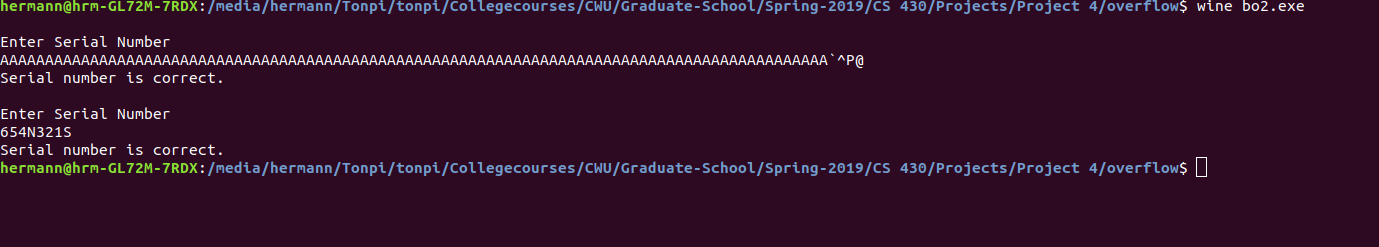
\includegraphics[width=\linewidth]{Problem_1.png}
				\captionof{figure}{Proof of Buffer Overflow Working for Problem 1}
				
			\subsubsection{Part2}
				Using a the disassembler $disasm.exe$ found from the internet, we found the serial number to be 654N321S
			
		\subsection{Problem 2}
		
			Using the program "part2.c" included in the submission package for this assignment, we found the serial number to be 8675309.
			
			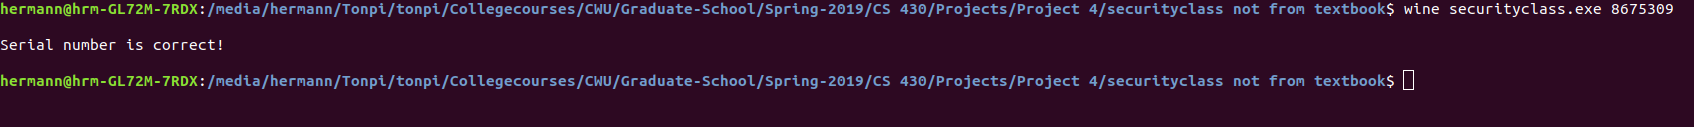
\includegraphics[width=\linewidth]{part2.png}
			\captionof{figure}{Proof of Serial Number working for Problem 2 }
			
			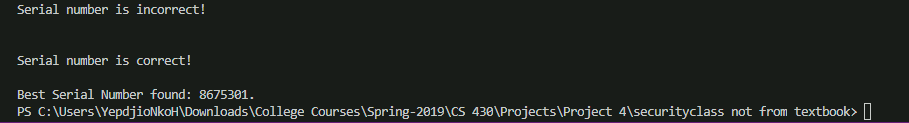
\includegraphics[width=\linewidth]{part2_2.png}
			\captionof{figure}{Output of part2.c}
			
		\section{Observations}
			As we can see from figure 3 above, the program part2.c finds only the first 6 digits of the serial number and for the last one, we either had to try all digits from  0 to 9 manually or alternatively starting from the last line on the output screen that says if the serial number is correct or not, we counted how many more lines we had to visit (moving upward) until we find a line that says "Serial number is correct!" and subtract that number from 9 to obtain the last digit for the serial number. In our case the last line was the correct line so, we had to visit zero more line in order to find that line. Therefore the last digit of the serial number was 9 - 0 = 9. 
			Another observation is that, part2.c might have to be run multiple times in order to get the correct serial number as the linearization approach relies on the trial time for each potential serial number and that time is not accurate. 
			
			
			
			
				
	
\end{document}